\documentclass{beamer}
\mode<presentation>
% \hypersetup{pdfpagemode=FullScreen}
\usepackage{amsmath}
\usepackage{amssymb}
%\usepackage{advdate}
\usepackage{adjustbox}
\usepackage{subcaption}
\usepackage{enumitem}
\usepackage{multicol}
\usepackage{mathtools}
\usepackage{listings}
\usepackage{url}
\def\UrlBreaks{\do\/\do-}
\usetheme{Boadilla}
\usecolortheme{lily}
\setbeamertemplate{footline}
{
  \leavevmode%
  \hbox{%
  \begin{beamercolorbox}[wd=\paperwidth,ht=2.25ex,dp=1ex,right]{author in head/foot}%
    \insertframenumber{} / \inserttotalframenumber\hspace*{2ex} 
  \end{beamercolorbox}}%
  \vskip0pt%
}
\setbeamertemplate{navigation symbols}{}

\providecommand{\nCr}[2]{\,^{#1}C_{#2}} % nCr
\providecommand{\nPr}[2]{\,^{#1}P_{#2}} % nPr
\providecommand{\mbf}{\mathbf}
\providecommand{\pr}[1]{\ensuremath{\Pr\left(#1\right)}}
\providecommand{\qfunc}[1]{\ensuremath{Q\left(#1\right)}}
\providecommand{\sbrak}[1]{\ensuremath{{}\left[#1\right]}}
\providecommand{\lsbrak}[1]{\ensuremath{{}\left[#1\right.}}
\providecommand{\rsbrak}[1]{\ensuremath{{}\left.#1\right]}}
\providecommand{\brak}[1]{\ensuremath{\left(#1\right)}}
\providecommand{\lbrak}[1]{\ensuremath{\left(#1\right.}}
\providecommand{\rbrak}[1]{\ensuremath{\left.#1\right)}}
\providecommand{\cbrak}[1]{\ensuremath{\left\{#1\right\}}}
\providecommand{\lcbrak}[1]{\ensuremath{\left\{#1\right.}}
\providecommand{\rcbrak}[1]{\ensuremath{\left.#1\right\}}}
\theoremstyle{remark}
\newtheorem{rem}{Remark}
\newcommand{\sgn}{\mathop{\mathrm{sgn}}}
\providecommand{\abs}[1]{\left\vert#1\right\vert}
\providecommand{\res}[1]{\Res\displaylimits_{#1}} 
\providecommand{\norm}[1]{\lVert#1\rVert}
\providecommand{\mtx}[1]{\mathbf{#1}}
\providecommand{\mean}[1]{E\left[ #1 \right]}
\providecommand{\fourier}{\overset{\mathcal{F}}{ \rightleftharpoons}}
%\providecommand{\hilbert}{\overset{\mathcal{H}}{ \rightleftharpoons}}
\providecommand{\system}{\overset{\mathcal{H}}{ \longleftrightarrow}}
	%\newcommand{\solution}[2]{\textbf{Solution:}{#1}}
%\newcommand{\solution}{\noindent \textbf{Solution: }}
\providecommand{\dec}[2]{\ensuremath{\overset{#1}{\underset{#2}{\gtrless}}}}
\newcommand{\myvec}[1]{\ensuremath{\begin{pmatrix}#1\end{pmatrix}}}
\let\vec\mathbf

\lstset{
%language=C,
frame=single, 
breaklines=true,
columns=fullflexible
}

\numberwithin{equation}{section}

\title[The Piece-wise Exponential]{The Piece-wise Exponential}
\author[Shiven Bajpai]{Shiven Bajpai}
\institute[AI24BTECH11030]{AI24BTECH11030\\IIT Hyderabad}

\date{\today} 
\begin{document}

\begin{frame}
\titlepage
\end{frame}

\begin{frame}
\tableofcontents
\end{frame}

\section{Problem}
\begin{frame}
\frametitle{Problem Statement}
Given that
\begin{align}
	f(t) &= e^{-at}u(t) + e^{bt}u(-t) \label{q1}\\
	u(t) &= \begin{cases}
		0, & t<0\\
		\frac{1}{2}, & t=0 \\
		1, & t>0
	\end{cases} \label{q2}\\
	\int_{-\infty}^{\infty} f(t) &= 1 \label{q3}
\end{align}

Find the possible values of $(a,b)$ if these are the end points of the latus recta of the associated conic. Plot $f(t)$ for these values of $(a,b)$
\end{frame}

\section{Solution}
\subsection{Finding the Conic}
\begin{frame}
\frametitle{Finding the Conic}

We expand the integral as 

\begin{align}
	\int_{-\infty}^{\infty} f(t) &= \int_{-\infty}^{0} f(t) + \int_{0}^{\infty} f(t)\\
	&= \int_{-\infty}^{0} e^{bt} + \int_{0}^{\infty} e^{-at}\\
	&= \frac{1}{b} + \frac{1}{a} \label{integral_result}
\end{align}

Subsituting \eqref{q3} in \eqref{integral_result}

\begin{align}
	\frac{1}{a} + \frac{1}{b} &= 1\\
	ab - a - b &= 0 \label{conic_ab}
\end{align}

Which is the equation of a conic.

\end{frame}

\subsection{Conversion to Standard Conic}
\begin{frame}
\frametitle{Conversion to Matrix equation}

If we take this conic to be of the form, and let $(a, b) = \vec{x}$

\begin{align}
	\text{g}(\vec{x}) = \vec{x}^\text{T}\vec{Vx} + 2\vec{u}^\text{T}\vec{x} + f \label{actual_conic}
\end{align}

By comparison we obtain:

\begin{center}
    \begin{tabular}{c c c}
        $\vec{V} = \myvec{0 & \frac{1}{2} \\ \frac{1}{2} & 0}$ &
    	$\vec{u} = \myvec{-\frac{1}{2} \\ -\frac{1}{2}}$ &
    	$f = 0$\\
    \end{tabular}
\end{center}

Clearly $\vec{V}$ is not of the form of a standard conic. So we will convert it using an affine transformation and then a reflection.
\end{frame}

\begin{frame}
\frametitle{Conversion to a Standard Conic}

Let $\vec{V} = \vec{PDP}^\text{T}$ (eigen-decomposition). First we apply the affine transformation 

\begin{align}
	\vec{x} &= \vec{Py} + \vec{c} \label{t1}
\end{align}

After this, we get the second eigenvalue as negative, so we use the orthogonal matrix for another transformation

\begin{align}
	\vec{y} &= \vec{P}_0\vec{z} \label{t2}
\end{align}

Here $\vec{P}_0$ is the reflection matrix $\myvec{0 & 1 \\ 1 & 0}$
    
\end{frame}

\subsection{Solving for solution}
\begin{frame}
    \frametitle{Enpoints of Latus Recta}
    
    Finally this gives us a standard conic as 

    \begin{align}
        \vec{z}^\text{T}\brak{\frac{\vec{D_0}}{f_0}}\vec{z} &= 1 \label{standard_conic}
    \end{align}

    Using standard formulae, we get the endpoints of latus rectum of standard conic ($\vec{\hat{z}}$) to be 

    \begin{align}
        \vec{\hat{z}} &= \myvec{\pm \sqrt{2} \\ \pm 2}
    \end{align}

    By reversing the transformations \eqref{t1} and \eqref{t2} we get the endpoints of the actual conic ($\vec{\hat{x}}$)

    \begin{center}
        \begin{tabular}{c c c c}
            $\vec{\hat{x}}_1 = \myvec{2+\sqrt{2} \\ \sqrt{2}}$
            $\vec{\hat{x}}_2 = \myvec{\sqrt{2} \\ 2+\sqrt{2}}$
            $\vec{\hat{x}}_3 = \myvec{2-\sqrt{2} \\ -\sqrt{2}}$
            $\vec{\hat{x}}_4 = \myvec{-\sqrt{2} \\ 2-\sqrt{2}}$
        \end{tabular}
    \end{center}
        
\end{frame}

\section{Plotting the Results}
\begin{frame}[fragile]
	\frametitle{Plotting the Conic}

	\begin{figure}[H]
		\centering
		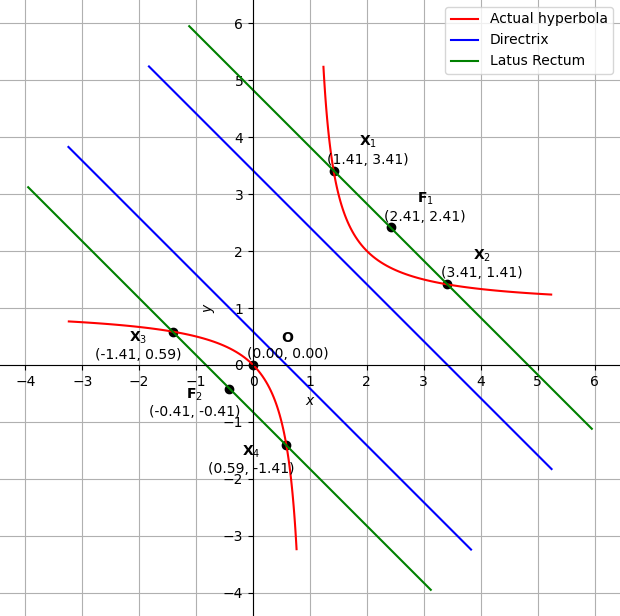
\includegraphics[width=0.65\textwidth]{Figures/Hyperbola.png}
	\end{figure}
	
\end{frame}

\begin{frame}[fragile]
	\frametitle{Plotting the Function}

    Out of these, $\vec{\hat{x}}_3$ and $\vec{\hat{x}}_4$ are unfit to be used as values for $(a, b)$ as the integral in \eqref{q3} will not converge. Plotting f(t) for the remaining two values of $(a,b)$ we get\\
    \bigskip

	\begin{figure}[H]
		\centering
		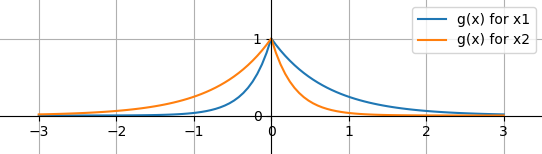
\includegraphics[width=0.9\textwidth]{Figures/function.png}
	\end{figure}
	
\end{frame}

\begin{frame}[fragile]
    \frametitle{References}

    The code for the plot and a fully detailed solution can be found at
	{\scriptsize
	\begin{lstlisting}
https://github.com/shivenBajpai/EE1030/blob/main/Misc/Documentation/main.pdf
https://github.com/shivenBajpai/EE1030/blob/main/Misc/Documentation/Codes/solution.py
	\end{lstlisting}
	}
    
\end{frame}

\section{Recreating the logo}
\begin{frame}
    \frametitle{Wait, What logo?}

    You may have noticed that the function in the last figure somewhat resembles sir's profile picture. That is because it is the same function.
    \bigskip
    
    Now we shall seek to recreate that logo.
\end{frame}

\subsection{Observing the original}
\begin{frame}[fragile]
    \frametitle{Observing the original}

    Before we can recreate sir's logo we must first extract some information from the original. Not only do we get the color information, we also find that:

    \begin{figure}[H]
		\centering
		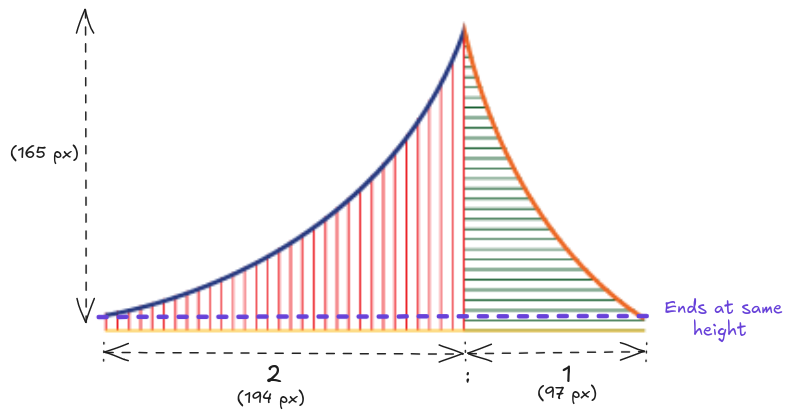
\includegraphics[width=0.95\textwidth]{Figures/anotated_original.png}
	\end{figure}

\end{frame}

\subsection{Recreation}
\begin{frame}[fragile]
    \frametitle{Recreation - Step I: Plot the curve}

    \begin{figure}[H]
		\centering
		\includegraphics[width=0.9\textwidth]{Figures/logo_1.png}
	\end{figure}

\end{frame}

\begin{frame}[fragile]
    \frametitle{Recreation - Step II: Add the lines}

    \begin{figure}[H]
		\centering
		\includegraphics[width=0.9\textwidth]{Figures/logo_2.png}
	\end{figure}

\end{frame}

\begin{frame}[fragile]
    \frametitle{Recreation - Step III: Scaling and Truncation}

    \begin{figure}[H]
		\centering
		\includegraphics[width=\textwidth]{Figures/logo_3.png}
	\end{figure}

\end{frame}

\begin{frame}[fragile]
    \frametitle{Recreation - Step IV: Clean it up}

    \begin{figure}[H]
		\centering
		\includegraphics[width=\textwidth]{Figures/logo.png}
	\end{figure}

\end{frame}

\section{A Note on File Formats}
\begin{frame}[fragile]
    \frametitle{A Note on File Formats}

    
    \begin{itemize}
        \only<1->{\item Images can be saved in multiple formats. For example .bmp, .jpg/.jpeg, .png, .svg}
        \bigskip
    
        \only<2->{
            \begin{center}
                \begin{tabular}{|c|c|c|c|c|}
                \hline
                 & .bmp & .jpeg & .png & .svg\\
                \hline
                Type & Raster & Raster & Raster & Vector\\
                \hline
                Compression & None & Lossy & Lossless & None$^\star$\\
                \hline
                Alpha Channel & No & No & Yes & N/A\\
                \hline
                Resolution & Fixed & Fixed & Fixed & Infinite\\
                \hline
            \end{tabular}
            \end{center}}
        \bigskip

        \only<3>{\item Matplotlib can output to all these formats, but you have to specify the transparent parameter of the savefig function as True}
    \end{itemize}


\end{frame}

\end{document}